%%%%%%%%%%%%%%%%%%%%%%%%%%%%%%%%%%%%%%%%%%
% Engineering problems / LaTeX Template
%		Semester 6
%		Institut d'Optique Graduate School
%%%%%%%%%%%%%%%%%%%%%%%%%%%%%%%%%%%%%%%%%%
%	6N-IntNum-BlocRobot	/ Embedded System
%%%%%%%%%%%%%%%%%%%%%%%%%%%%%%%%%%%%%%%%%%
%
% Created by:
%	Julien VILLEMEJANE - 19/oct/2024	
%
%%%%%%%%%%%%%%%%%%%%%%%%%%%%%%%%%%%%%%%%%%
% Professional Newsletter Template
% LaTeX Template
% Version 1.0 (09/03/14)
%
% Created by:
% Bob Kerstetter (https://www.tug.org/texshowcase/) and extensively modified by:
% Vel (vel@latextemplates.com)
% 
% This template has been downloaded from:
% http://www.LaTeXTemplates.com
%
% License:
% CC BY-NC-SA 3.0 (http://creativecommons.org/licenses/by-nc-sa/3.0/)
%
%%%%%%%%%%%%%%%%%%%%%%%%%%%%%%%%%%%%%%%%%

\documentclass[a4paper,11pt,titlepage]{article} % The default font size is 10pt; 11pt and 12pt are alternatives

%%%%%%%%%%%%%%%%%%%%%%%%%%%%%%%%%%%%%%%%%%%%%%%%%%%%%%%%%%%%%%%%%%%%%%%%%%%%%%%%%%%%%%%%%%%%%%%%%%%%%%%%%%%%%%%%%%%%%%%%%%%%%%%%%%%%%%%%%%%%%%%%%%%%%%%%%%%%%%%%%%%%%%%%%%%%%%%%%%%%%%%%%%%%%%%%%%%%%%%%%%%%%%%%%%%%%%%%%%%%%%%%%%%%%%%%%%%%%%%%%%%%%%%%%%%%
\usepackage{opto_elec_villemejane}

%%%%%%%%%%%%%%%%%%%%%%%%%%%%%%%%%%%%%%%%%%%%%%%%
%%%%%%%%%%%%%%%%%%%%%%%%%%%%%%%%%%%%%%%%%%%%%%%%
\begin{document}



% Page de garde
\begin{titlepage}

\begin{center}
	\begin{minipage}{2.5cm}
	\begin{center}
		
\includegraphics[width=8cm]{images/Logo-LEnsE.png}
	\end{center}
\end{minipage}\hfill
\begin{minipage}{10cm}
	\begin{center}
	\textbf{Institut d'Optique Graduate School }\\[0.1cm]
    \textbf{Interfaçage Numérique}


	\end{center}
\end{minipage}\hfill


\vspace{4cm}


{\huge \bfseries \textsc{Interfaçage Numérique}} \\[0.5cm]
{\large \bfseries Travaux Pratiques} \\[0.2cm]
Semestre 6

\vspace{2cm}
% Title
\rule{\linewidth}{0.3mm} \\[0.4cm]
{ \huge \bfseries\color{violet_iogs} Keil uVision / STM32 / MBED-OS\\[0.4cm] }
\rule{\linewidth}{0.3mm} \\[1cm]

1 séance

\bigskip

\begin{center}
%	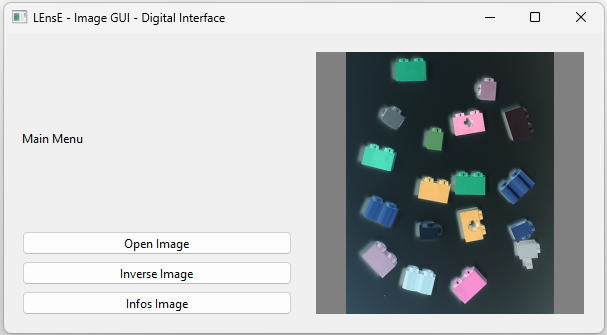
\includegraphics[width=0.5\textwidth]{images/image_gui.png}
\end{center}

\vfill

\textit{Ce sujet est disponible au format électronique sur le site du LEnsE - https://lense.institutoptique.fr/ dans la rubrique Année / Première Année / Interfaçage Numérique S6 / Bloc 1 Systèmes embarqués / Intro MBED et STM32.}

\rule{\linewidth}{0.3mm} \\[1cm]

\textit{\large Des \textbf{bibliothèques de fonctions} pour certains composants sont disponibles à l'adresse suivante :}

\medskip

\href{https://github.com/IOGS-Digital-Methods/keil_stm32/tree/main/MBED_os/libs}{\large https://github.com/IOGS-Digital-Methods/keil\_stm32/tree/main/MBED\_os/libs}

\medskip

\textit{dépôt GitHub - bibliothèques validées sous \textbf{MBED-OS 6.17}}

\textit{Une version est également disponible dans le répertoire S:/mbed\_keil/ des PC de la salle de TP.}

% Bottom of the page
%{\textbf{\large {Année universitaire} 2024-2025}}

\end{center}
\end{titlepage}


\newpage
\strut % empty page
\newpage
\strut % empty page
%%%%%%%%%%%%%%%%%%%%%%%%%%%%%%%%%%%%%%%%%%%%%%%%
%%%%%%%%%%%%%    Séance 1 détaillée

\begin{minipage}[c]{.25\linewidth}
	
\includegraphics[width=4cm]{images/Logo-LEnsE.png}
\end{minipage} \hfill
\begin{minipage}[c]{.4\linewidth}

\begin{center}
\vspace{0.3cm}
{\Large \textsc{Interfaçage Numérique}}

\medskip

6N-047-SCI \qquad \textbf{\Large Bloc MBED}

\end{center}
\end{minipage}\hfill

\vspace{0.5cm}

\noindent \rule{\linewidth}{1pt}

{\noindent\Large \rule[-7pt]{0pt}{30pt} Séance 1 / MBED et Nucléo-STM32 (sans maquette !!)} 

\noindent \rule{\linewidth}{1pt}


%%%%%%%%%%%%%%%%%%%%%%%%%%%%%%%%%%%%%%%%%%%%%%%%
%%%%%%%%%%%%%    Objectifs
\section{Objectifs de la séance}

Cette première séance est consacrée à la découverte de la \textbf{programmation de systèmes embarqués} (ici des cartes \textbf{Nucléo} de \textit{STMicroelectronics}, basées sur des microcontroleurs \textit{STM32}) et la prise en main de l'interface de développement \textbf{Keil Studio Cloud} (et les bibliothèques MBED).


	\begin{description}
		\item[Etape 0 - 30 min] Tester un premier programme
		\item[Etape 1 - 45 min] Piloter des sorties numériques - LED
		\item[Etape 2 - 45 min] Acquérir des données numériques - Bouton-poussoirs
		\item[Etape 3 - 45 min] Mettre en \oe{}uvre des interruptions sur des événements externes
		\item[Etape 4 - 45 min] Utiliser des sorties modulées en largeur d'impulsion (PWM) - LEDs
		\item[Etape 5 - 60 min] Acquérir des données analogiques - Potentiomètre
	\end{description}	


%%%%%%%%%%%%%%%%%%%%%%%%%%%%%%%%%%%%%%%%%%%%%%%%
%%%%%%%%%%%%%    Arduino
\subsection{IDE Keil uVision et MBED-OS}

\textbf{Mbed-OS} est un système d'exploitation (\textit{Operating System}) pour des \textbf{systèmes embarqués}, conçu pour des \textbf{microcontroleurs de type ARM}. Cet ensemble de bibliothèques permet une abstraction des couches matérielles de bas niveau du microcontroleur. 

La division \textbf{Keil} de Arm fourni un environnement de développement, nommé \textbf{Keil uVision}, pour des projets basés sur des microcontroleurs STM32

\href{https://www.keil.arm.com/}{https://www.keil.arm.com/}


%%%%%%%%%%%%%%%%%%%%%%%%%%%%%%%%%%%%%%%%%%%%%%%%
%%%%%%%%%%%%%    Nucleo
\subsection{Carte Nucleo-STM32}

Les cartes Nucleo sont des \textbf{plateformes de développement} basées sur les \textbf{microcontrôleurs STM32} de \textit{STMicroelectronics}. Elles sont conçues pour faciliter le prototypage et le développement de projets embarqués, similaires aux cartes Arduino, mais elles sont souvent utilisées pour des applications plus complexes et performantes.


\begin{center}
	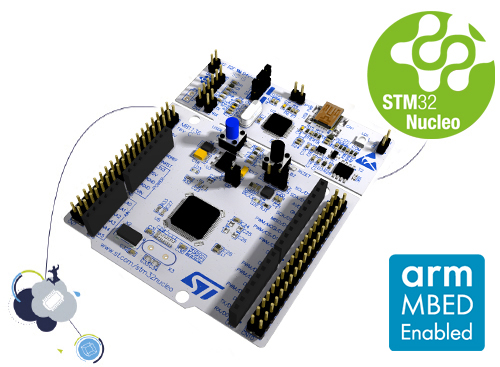
\includegraphics[width=0.2\textwidth]{images/nucleo_board.jpg}
\end{center}

Elles sont équipées d'un débogueur ST-LINK intégré, ce qui permet de programmer et de déboguer le microcontrôleur directement sans matériel additionnel.

\textsl{Le brochage de la carte Nucleo L476RG est fournie en annexe à ce document} : \hyperref[doc:nucleo_pins_476RG]{Brochage Nucléo L476RG}


\cleardoublepage


{\large \textbf{ATTENTION}} 

\textit{La procédure décrite ici ne fonctionne que pour une installation très spécifique des différentes ressources, celles mises en place à l'Institut d'Optique - salles de TP d'électronique. La procédure d'installation est décrite à l'adresse suivante : }

\href{https://github.com/IOGS-Digital-Methods/keil_stm32/blob/main/MBED_os/README.md}{https://github.com/IOGS-Digital-Methods/keil\_stm32/blob/main/MBED\_os/README.md}

\bigskip


Une \textbf{série d'exemples de code} (ainsi qu'une code de base) est disponible à l'adresse suivante : 

\href{https://github.com/IOGS-Digital-Methods/keil_stm32}{https://github.com/IOGS-Digital-Methods/keil\_stm32}

dans la section MBED\_os / boards / L476RG.

%%%%%%%%%%%%%%%%%%%%%%%%%%%%%%%%%%%%%%%%%%%%%%%%
%%%%%%%%%%%%%    Premier programme
\section{Etape 0 / Tester un premier programme}


\subsection{Télécharger le projet de base}

Avant de pouvoir programmer le microcontroleur présent sur les cartes Nucléo que nous allons utiliser, il faut au préalable \textbf{avoir un projet} pour \textsl{Keil uVision}.

Un exemple de base (en version archivée) est disponible au téléchargement ici : 

\href{https://lense.institutoptique.fr/ressources/mbed/hello-L476RG.zip}{https://lense.institutoptique.fr/ressources/mbed/hello-L476RG.zip}

\Manip Télécharger le fichier précédent et décompresser l'archive dans un répertoire de votre ordinateur.

\subsection{Changer le nom du projet (facultatif)}

\Manip Dans le répertoire décompressé, renommer les fichiers (opération facultative) :

\begin{itemize}
	\item \textsl{hello-L476RG.uvprojx} en \textsl{nom\_de\_votre\_projet.uvprojx}
	\item \textsl{hello-L476RG.uvoptx} en \textsl{nom\_de\_votre\_projet.uvoptx}
\end{itemize}

\Manip A l'aide d'un éditeur de texte (Notepad++ par exemple), ouvrir le fichier \textsl{nom\_de\_votre\_projet.uvprojx} puis remplacer toutes les occurences de \textsl{hello-L476RG} par \textsl{nom\_de\_votre\_projet}. (opération facultative)


\subsection{Lancer Keil uVision}

\Manip Dans le répertoire décompressé, double-cliquer sur le fichier dont l'extension est \textbf{*.uvprojx}. Le logiciel \textit{Keil uVision} s'ouvre.

\begin{center}
	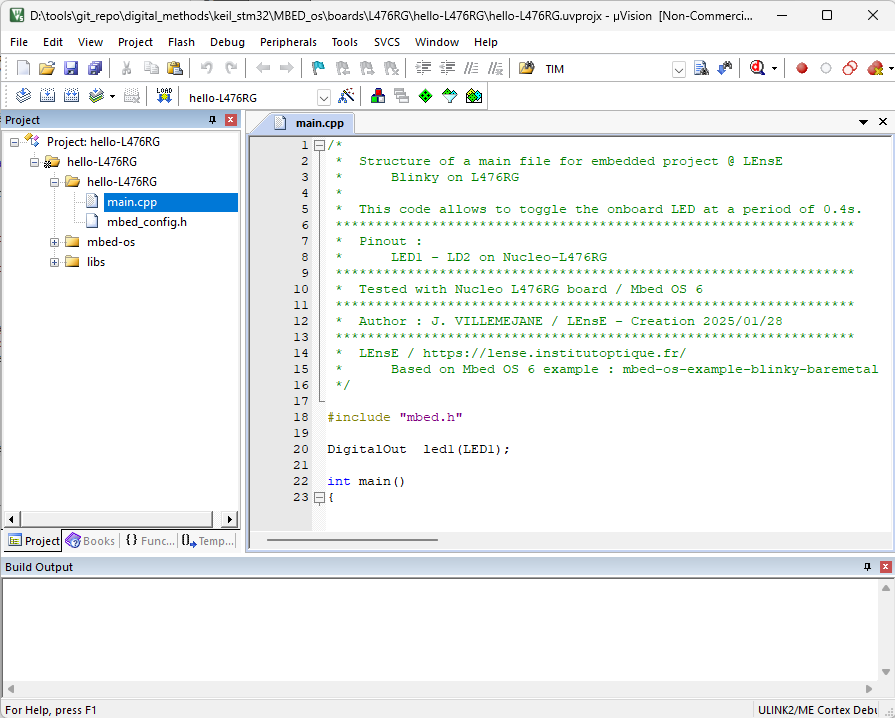
\includegraphics[width=0.5\textwidth]{images/uvision_interface.png}
\end{center}


\newpage
\subsection{Programme Blinky (baremetal)}

Le code principal se trouver dans le fichier \textsl{\textbf{main.cpp}}, que vous pouvez retrouver dans la zone de droite de l'interface.

Le programme \textsl{\textbf{main.cpp}} ressemble à celui-ci :

\begin{lstlisting}
#include "mbed.h"

#define WAIT_TIME_MS 500 
DigitalOut led1(LED1);

int main()
{
    printf("Hello L476RG - LEnsE !!\r\n");

    while (1)
    {
        led1 = !led1;
        thread_sleep_for(WAIT_TIME_MS);
    }
}

\end{lstlisting}

\textit{Sur la carte Nucléo la sortie LED1 correspond à la LED nommée LD2.}

Le langage utilisé par l'environnement MBED est un langage proche du C++. Le programme ainsi écrit doit nécessairement \textbf{être compilé} avant de pouvoir \textbf{être téléversé} sur la carte où il sera ensuite \textbf{exécuté}.

\subsection{Structure du code}

Un programme embarqué est constitué de \textbf{deux étapes principales} : 

\begin{itemize}
	\item une \textbf{initialisation} : exécutée une fois à la mise sous tension de la carte ou lors de l'appui sur le bouton Reset.
	\item une \textbf{boucle infinie} : exécutée de manière infinie. Cette boucle a pour principale mission, sur un système embarqué, de récupérer les valeurs des entrées, de calculer les valeurs des sorties et de mettre à jour les sorties.
\end{itemize}

\begin{center}
	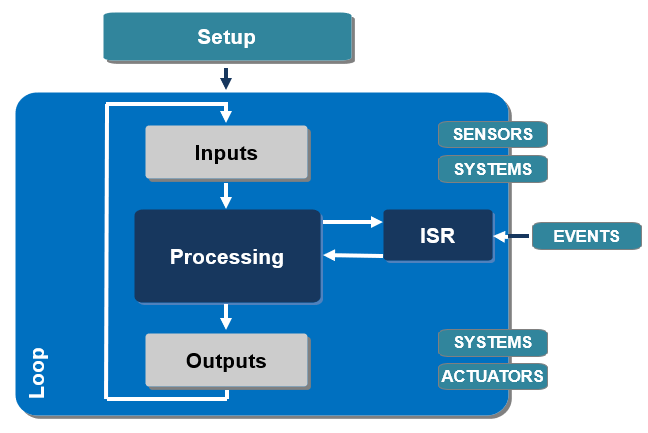
\includegraphics[width=0.5\textwidth]{images/arduino_program_structure.png}
\end{center}

\textit{D'autres étapes sont possibles lorsqu'on autorise le fonctionnement par interruption (voir dans la suite de ce document).}


\subsection{Compilation}

Le programme fourni est fonctionnel. Il suffit de le compiler. Pour cela, cliquer sur la seconde icône de la barre d'action :

\begin{center}
	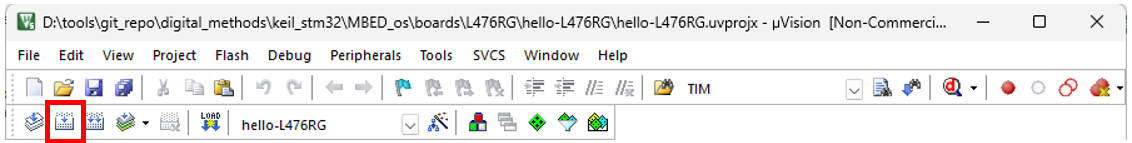
\includegraphics[width=0.8\textwidth]{images/uvision_compile.png}
\end{center}

A la fin de cette étape, si la compilation s'est terminée avec succès, un fichier binaire est créé.

\bigskip

\textbf{Remarque} \textit{La première compilation du projet peut être longue. L'intégralité des bibliothèques doit être compilée.}


\subsection{Téléversement du programme}

La carte doit être connectée à l'ordinateur via le port USB adéquat. Les cartes Nucléo sont reconnues comme des supports de stockage amovible.

Il suffit alors de déplacer le fichier binaire obtenu après la compilation dans le support de stockage. Ce fichier se trouve dans le répertoire du projet. Il porte l'extension \textbf{*.bin}.

\bigskip

\textbf{Attention !} Le fichier va automatiquement disparaître du stockage. Il sera cependant bien téléverser dans la carte Nucléo (LED clignotante au niveau du port USB de la carte Nucléo).

\bigskip

\textbf{Attention !} Il est parfois nécessaire de cliquer sur le bouton \textit{Reset} (bouton noir) sur la carte Nucléo pour faire démarrer le programme. Et parfois débrancher et rebrancher le câble USB...


\bigskip

\textbf{Il est conseillé de repartir du projet de base pour chaque nouveau projet que vous réaliserez.}


\cleardoublepage
%%%%%%%%%%%%%%%%%%%%%%%%%%%%%%%%%%%%%%%%%%%%%%%%
%%%%%%%%%%%%%    Premier programme
\section{Etape 1 / Piloter des sorties numériques - LED}

Afin de pouvoir interagir avec le monde extérieur, les microcontrôleurs disposent d'un ensemble d'\textbf{entrées} et de \textbf{sorties}. 

Chacune de ces entrées-sorties portent un nom, au format \textsc{Px\_n}, où \textsc{x} est le nom du port (A, B...) et \textsc{n} le numéro de la broche.

\begin{center}
	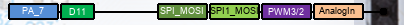
\includegraphics[width=0.5\textwidth]{images/nucleo_pin_functions.png}
	
	Exemple de la broche PA\_7 (port A, broche 7)
\end{center}


\subsection{Choix d'une broche}

Toutes les broches peuvent être utilisées en \textbf{entrée} ou en \textbf{sortie} \textbf{numérique}, c'est à dire un type de signal qui ne peut prendre que \textbf{deux états} : haut ou bas (aussi appelés 1 ou 0, ou encore \textit{HIGH} et \textit{LOW} en Arduino). 

\textit{Certaines broches ont également d'autres fonctionnalités : entrées analogiques, sorties modulées PWM, communication série...}


\subsection{Câblage d'une LED}

Nous allons voir ici comment connecter une LED à la carte Nucléo sur la broche D10 par exemple de la carte (ou PB\_6 - port B, broche 6).

Les schémas de câblage possibles sont les suivants :

\begin{center}
	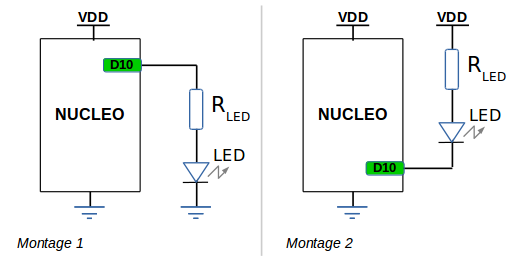
\includegraphics[width=0.7\textwidth]{images/MINE_Nucleo_LED_Connexion.png}
	
	Exemple de la broche D10 reliée à une LED (ou PB\_6 - port B, broche 6)
\end{center}

Dans le cas des cartes Nucléo, la tension $\operatorname{VDD}$ est égale à $3.3\operatorname{V}$.

Il est indispensable d'associer la LED à une \textbf{résistance de protection}, permettant de limiter le courant : 

$$R_{LED} > \frac{VDD - V_{F}}{I_{Fmax}}$$

\textit{Les valeurs $V_F$ et $I_{Fmax}$ dépendent de la LED utilisée et sont à chercher dans sa documentation technique.}


\subsection{Programme}

\subsubsection{Paramétrage}

Pour \textbf{configurer une broche en sortie}, il faut ajouter l'instruction suivante \textbf{en dehors de toute fonction} (où \textsl{D10} est le nom d'une broche du composant) :

\begin{lstlisting}
DigitalOut led2(PB_6);
\end{lstlisting}

\textsl{led2} correspond au nom de la variable assignée à la broche \textsc{D10}.

\subsubsection{Utilisation}

Pour \textbf{affecter une valeur à une broche en sortie}, il faut utiliser une des deux instructions suivantes (où \textsl{led2} est le nom de la variable associée à la broche du composant) selon que l'on veut mettre la sortie à l'état bas (\textit{0}) ou à l'état haut (\textit{1}) :

\begin{lstlisting}
led2 = 0;
led2 = 1;
\end{lstlisting}


\subsection{Travail à réaliser}

\Manip Créer un nouveau projet basé sur l'exemple \textbf{\textsl{hello-L476RG}}.

\Manip Réaliser un programme qui permet d'allumer deux LEDs rouges cablées sur les sorties D10 et D11. Les LEDs devront s'allumer de manière complémentaire chaque seconde.

\newpage
%%%%%%%%%%%%%%%%%%%%%%%%%%%%%%%%%%%%%%%%%%%%%%%%
%%%%%%%%%%%%%    Premier programme
\section{Etape 2 / Acquérir des données numériques - Bouton-poussoirs}


\subsection{Câblage d'un bouton-poussoir}

Nous allons voir ici comment brancher un bouton-poussoir à la carte Nucléo sur la broche D7 par exemple de la carte (ou PA8 - port A, broche 8).

Le schéma de câblage est le suivant :

\begin{center}
	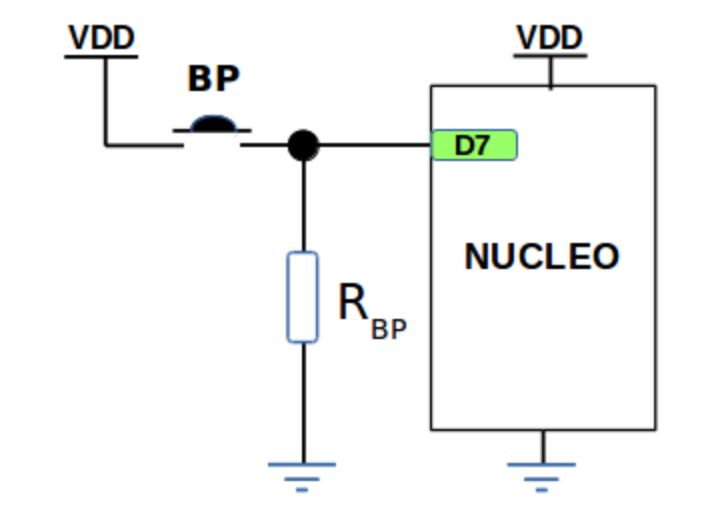
\includegraphics[width=0.4\textwidth]{images/MINE_Nucleo_BoutonPoussoir.png}
	
	Exemple de la broche D7 reliée à un bouton-poussoir (ou PA\_8 - port A, broche 8)
\end{center}

Avant de câbler la sortie du bouton-poussoir à l'entrée de la carte, vérifier que vous avez bien une tension de $0\operatorname{V}$ (lorsque le bouton-poussoir n'est pas activé) et une tension de $3.3\operatorname{V}$ (dans l'autre cas).

\subsection{Programme}

\subsubsection{Paramétrage}

Pour \textbf{configurer une broche en entrée}, il faut ajouter l'instruction suivante \textbf{en dehors de toute fonction} :

\begin{lstlisting}
DigitalIn  sw1(PA_8);
\end{lstlisting}

\subsubsection{Utilisation}

Pour \textbf{récupérer une valeur d'une entrée}, il faut utiliser l'instruction suivante :

\begin{lstlisting}
int bpVal = sw1;
\end{lstlisting}

La variable \textsl{bpVal} peut valoir \textsc{1} ou \textsc{0} selon l'état du bouton-poussoir (ou de l'entrée).

\subsection{Travail à réaliser}

\Manip Créer un nouveau projet basé sur l'exemple \textbf{\textsl{hello-L476RG}}.

\Manip Réaliser un programme qui permet d'allumer chacune des LEDs rouges précédentes à l'aide de deux bouton-poussoirs cablés sur les entrées D6 et D7 (un bouton-poussoir par LED).


\newpage
%%%%%%%%%%%%%%%%%%%%%%%%%%%%%%%%%%%%%%%%%%%%%%%%
%%%%%%%%%%%%%    Premier programme
\section{Etape 3 / Mettre en \oe{}uvre des interruptions sur des événements externes}

\subsection{Scrutation}

La \textbf{scrutation} (ou \textit{polling} en anglais) est une méthode de \textbf{vérification régulière de l'état des périphériques ou des capteurs} dans un système embarqué pour détecter si un événement spécifique s'est produit. 

Dans ce contexte, le programme principal exécute une boucle continue (fonction \textsl{loop()} sous Arduino) où il interroge périodiquement chaque périphérique pour voir s'il nécessite une action. 

\begin{center}
	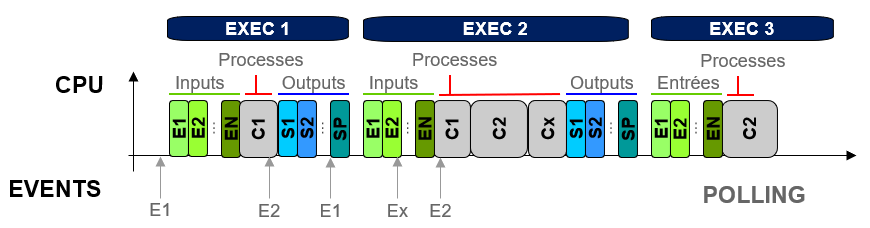
\includegraphics[width=0.8\textwidth]{images/gen_polling.png}
\end{center}

La \textbf{scrutation} ne permet pas de gérer d'un événement rapidement et monopolise le microcontrôleur pour vérifier constamment l'état des capteurs ou des périphériques.


\subsection{Interruptions}

Une \textbf{interruption} est un signal envoyé au microcontrôleur pour lui demander d'\textbf{arrêter temporairement l'exécution de son programme principal} et de \textbf{s'occuper d'une tâche prioritaire spécifique}. Lorsque l'interruption est terminée, le microcontrôleur reprend son programme là où il s'était arrêté.

\begin{center}
	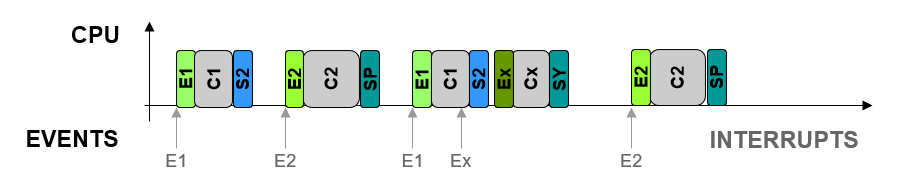
\includegraphics[width=0.8\textwidth]{images/gen_isr.png}
\end{center}


Cette méthode permet au système de \textbf{réagir rapidement à des événements externes} - changement de signal sur une broche, compteur qui atteint une certaine valeur - sans avoir besoin de vérifier constamment si l'événement a eu lieu, contrairement à la scrutation. 

Pour en savoir plus sur les interruptions, vous pouvez consulter le document à l'adresse suivante :

\href{https://iogs-lense-training.github.io/nucleo-basics/contents/polling_interrupts_rtos.html}{https://iogs-lense-training.github.io/nucleo-basics/contents/polling\_interrupts\_rtos.html}

\textit{Les interruptions sont également souvent utilisées dans les applications où un timing précis est nécessaire (par exemple, un compteur de temps).}


\subsubsection{Paramétrage}

Pour \textbf{configurer une broche en entrée permettant une interruption}, il faut ajouter l'instruction suivante \textbf{en dehors de toute fonction} :

\begin{lstlisting}
InterruptIn   sw1(PA_8);
\end{lstlisting}

\medskip

Il existe 2 modes possibles pour les interruptions sur des signaux externes (entrées numériques) : 

\begin{itemize}
	\item \textbf{rise} - front montant d'un signal
	\item \textbf{fall} - front descendant d'un signal
\end{itemize}

\medskip

Il faut ensuite paramétrer l'action à réaliser lors d'un événements sur cette entrée.

Pour cela, il faut ajouter l'instruction suivante au début de la fonction \textsl{main()} (phase d'initialisation) :

\begin{lstlisting}
sw1.rise(&sw_ISR);
\end{lstlisting}

où \textsl{sw\_ISR()} est une fonction, appelée \textbf{routine d'interruption}.

\subsubsection{Routine d'interruption}

Une \textbf{routine d'interruption}, aussi appelée \textbf{ISR} (\textit{Interrupt Service Routine}), est la fonction qui s'exécute automatiquement en réponse à une interruption. 

C'est une fonction classique, mais qui ne retourne pas de donnée.

\begin{lstlisting}
void sw_ISR(void){
  bool led_state = led1;
  led1 = !led_state;
} 
\end{lstlisting}

Dans cet exemple, à chaque front descendant sur l'entrée \textsl{PA\_8}, la fonction \textsl{sw\_ISR()} est appelée. Elle lit alors l'état de la sortie \textsl{led1} pour ensuite l'inverser.

\subsection{Travail à réaliser}

On se propose de tester le code \textsl{interrupt\_on\_input.cpp}. Ce fichier est disponible sur le site du LEnsE dans la rubrique \textit{Année / Première Année / Interfaçage Numérique S6 / Bloc 1 Systèmes embarqués / Exemples MBED pour STM32}.

\Manip Tester le code fourni. 

\Quest A quel moment est appelée la fonction \textsl{sw\_ISR()} ?

\Manip Réaliser un programme qui permet d'allumer à l'aide d'un premier interrupteur, câblé sur l'entrée D7, une LED câblée sur la sortie D10 et de l'éteindre à l'aide d'un second interrupteur câblé sur l'entrée D6. \textbf{Votre programme devra utiliser uniquement le principe d'interruption.}


\newpage
%%%%%%%%%%%%%%%%%%%%%%%%%%%%%%%%%%%%%%%%%%%%%%%%
%%%%%%%%%%%%%    Premier programme
\section{Etape 4 / Utiliser des sorties modulées en largeur d'impulsion (PWM) - LEDs}

La \textbf{modulation en largeur d'impulsions} (MLI ou \textit{PWM – Pulsed Witdh Modulation} – en anglais) est une méthode permettant de générer un signal rectangulaire de \textbf{période $T$ fixe} (ou de fréquence $1/T$ fixe) et dont le \textbf{rapport cyclique}, i.e. le rapport du temps haut $t_h$ sur la période, noté $RC = \frac{t_
h}{T}$, est variable.

\begin{center}
	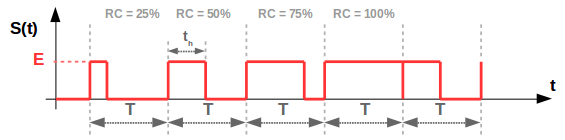
\includegraphics[width=0.6\textwidth]{images/MINE_ElecNum_PWM_SignalPrincipe.png}
\end{center}

\subsection{Choix de la broche de sortie}

Toutes les broches du microcontroleur ne sont pas utilisables comme sortie modulée en largeur d'impulsion. Cela nécessite l'utilisation de modules internes spécifiques (\textit{timer} et comparateur notamment).

Il faut choisir une broche où le terme \textit{PWM} est mentionné.

\begin{center}
	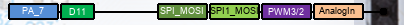
\includegraphics[width=0.5\textwidth]{images/nucleo_pin_functions.png}
	
	Exemple de la broche PA\_7 (port A, broche 7), utilisable en PWM
\end{center}

\subsection{Travail à réaliser}


On se propose de tester le code \textsl{pwm\_fade.cpp}. Ce fichier est disponible sur le site du LEnsE dans la rubrique \textit{Année / Première Année / Interfaçage Numérique S6 / Bloc 1 Systèmes embarqués / Exemples MBED pour STM32}.

\Manip Tester le code fourni. 

\Manip Visualiser à l'aide d'un oscilloscope le signal électrique appliqué sur la LED.

\Quest Expliquer le principe de fonctionnement de ce système.

\Manip Réaliser un programme qui permet de modifier la luminosité de la LED câblée sur la sortie D7 à l'aide des deux bouton-poussoirs, câblés sur D10 et D11 (un pour augmenter, l'autre pour diminuer la luminosité). \textbf{Votre programme devra utiliser uniquement le principe d'interruption.}


\newpage
%%%%%%%%%%%%%%%%%%%%%%%%%%%%%%%%%%%%%%%%%%%%%%%%
%%%%%%%%%%%%%    Premier programme
\section{Etape 5 / Acquérir des données analogiques - Potentiomètre}

Sur les systèmes numériques, et les microcontrôleurs en particulier, les broches sont naturellement des entrées/sorties numériques.

Or, la plupart des signaux qui nous entourent et que l'on cherche à mesurer (luminosité, température, vitesse...) sont des \textbf{grandeurs analogiques}. Pour palier à ce problème, la plupart des fabricants de microcontrôleurs ont intégré des \textbf{convertisseurs analogiques-numériques} (\textit{ADC – Analog to Digital Converter}) à leur système, afin d'éviter de passer par des composants externes.


\subsection{Câblage d'un potentiomètre}

Afin de pouvoir générer une tension analogique dont la tension est variable, nous allons utiliser un potentiomètre.

\begin{center}
	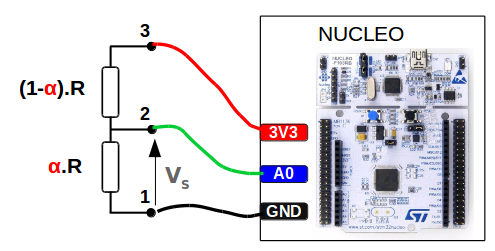
\includegraphics[width=0.6\textwidth]{images/MINE_Nucleo_CablagePotentiometre.png}
\end{center}


\subsection{Travail à réaliser}

\Manip Câbler un potentiomètre de $10\operatorname{k\Omega}$ entre $0\operatorname{V}$ et $3.3\operatorname{V}$, sur ses broches 1 et 3. Vérifier que la broche 2 varie selon la position du curseur de $0\operatorname{V}$ à $3.3\operatorname{V}$.

\textit{On pourra utiliser la sortie $3.3\operatorname{V}$ et la référence \textit{GND} de la carte Nucléo pour alimenter le potentiomètre.}

\bigskip

On se propose de tester le code \textsl{analog\_in.cpp}. Ce fichier est disponible sur le site du LEnsE dans la rubrique \textit{Année / Première Année / Interfaçage Numérique S6 / Bloc 1 Systèmes embarqués / Exemples MBED pour STM32}.

\Manip Tester le code fourni. Le potentiomètre devra être relié à l'entrée A0 de la carte Nucléo.

\Manip Utiliser le logiciel \textbf{TeraTerm} pour visualiser les messages transmis à la carte Nucléo via l'instruction \textsl{printf()}.

\Quest Expliquer le fonctionnement de ce code.

\Manip Réaliser un programme qui permet de modifier la luminosité de la LED câblée sur la sortie D7 à l'aide de la valeur convertie du potentiomètre. Attention au type des variables... \textit{int} ou \textit{float} !

\bigskip


\noindent \rule{\linewidth}{1pt}

\begin{center}
\Large
D'autres tutoriels sont disponibles à l'adresse suivante :

https://lense.institutoptique.fr/nucleo/
\end{center}


\newpage
%%%%%%%%%%%%%%%%%%%%%%%%%%%%%%%%%%%%%%%%%%%%%%%%
%%%%%%%%%%%%%    Premier programme
\section*{Annexe - Compléments de langage C++}

\subsection*{Fonction main()}

\subsection*{Typage des données}

\subsection*{Affichage sur la console}

\subsection*{Utilisation d'un tableau}



\newpage
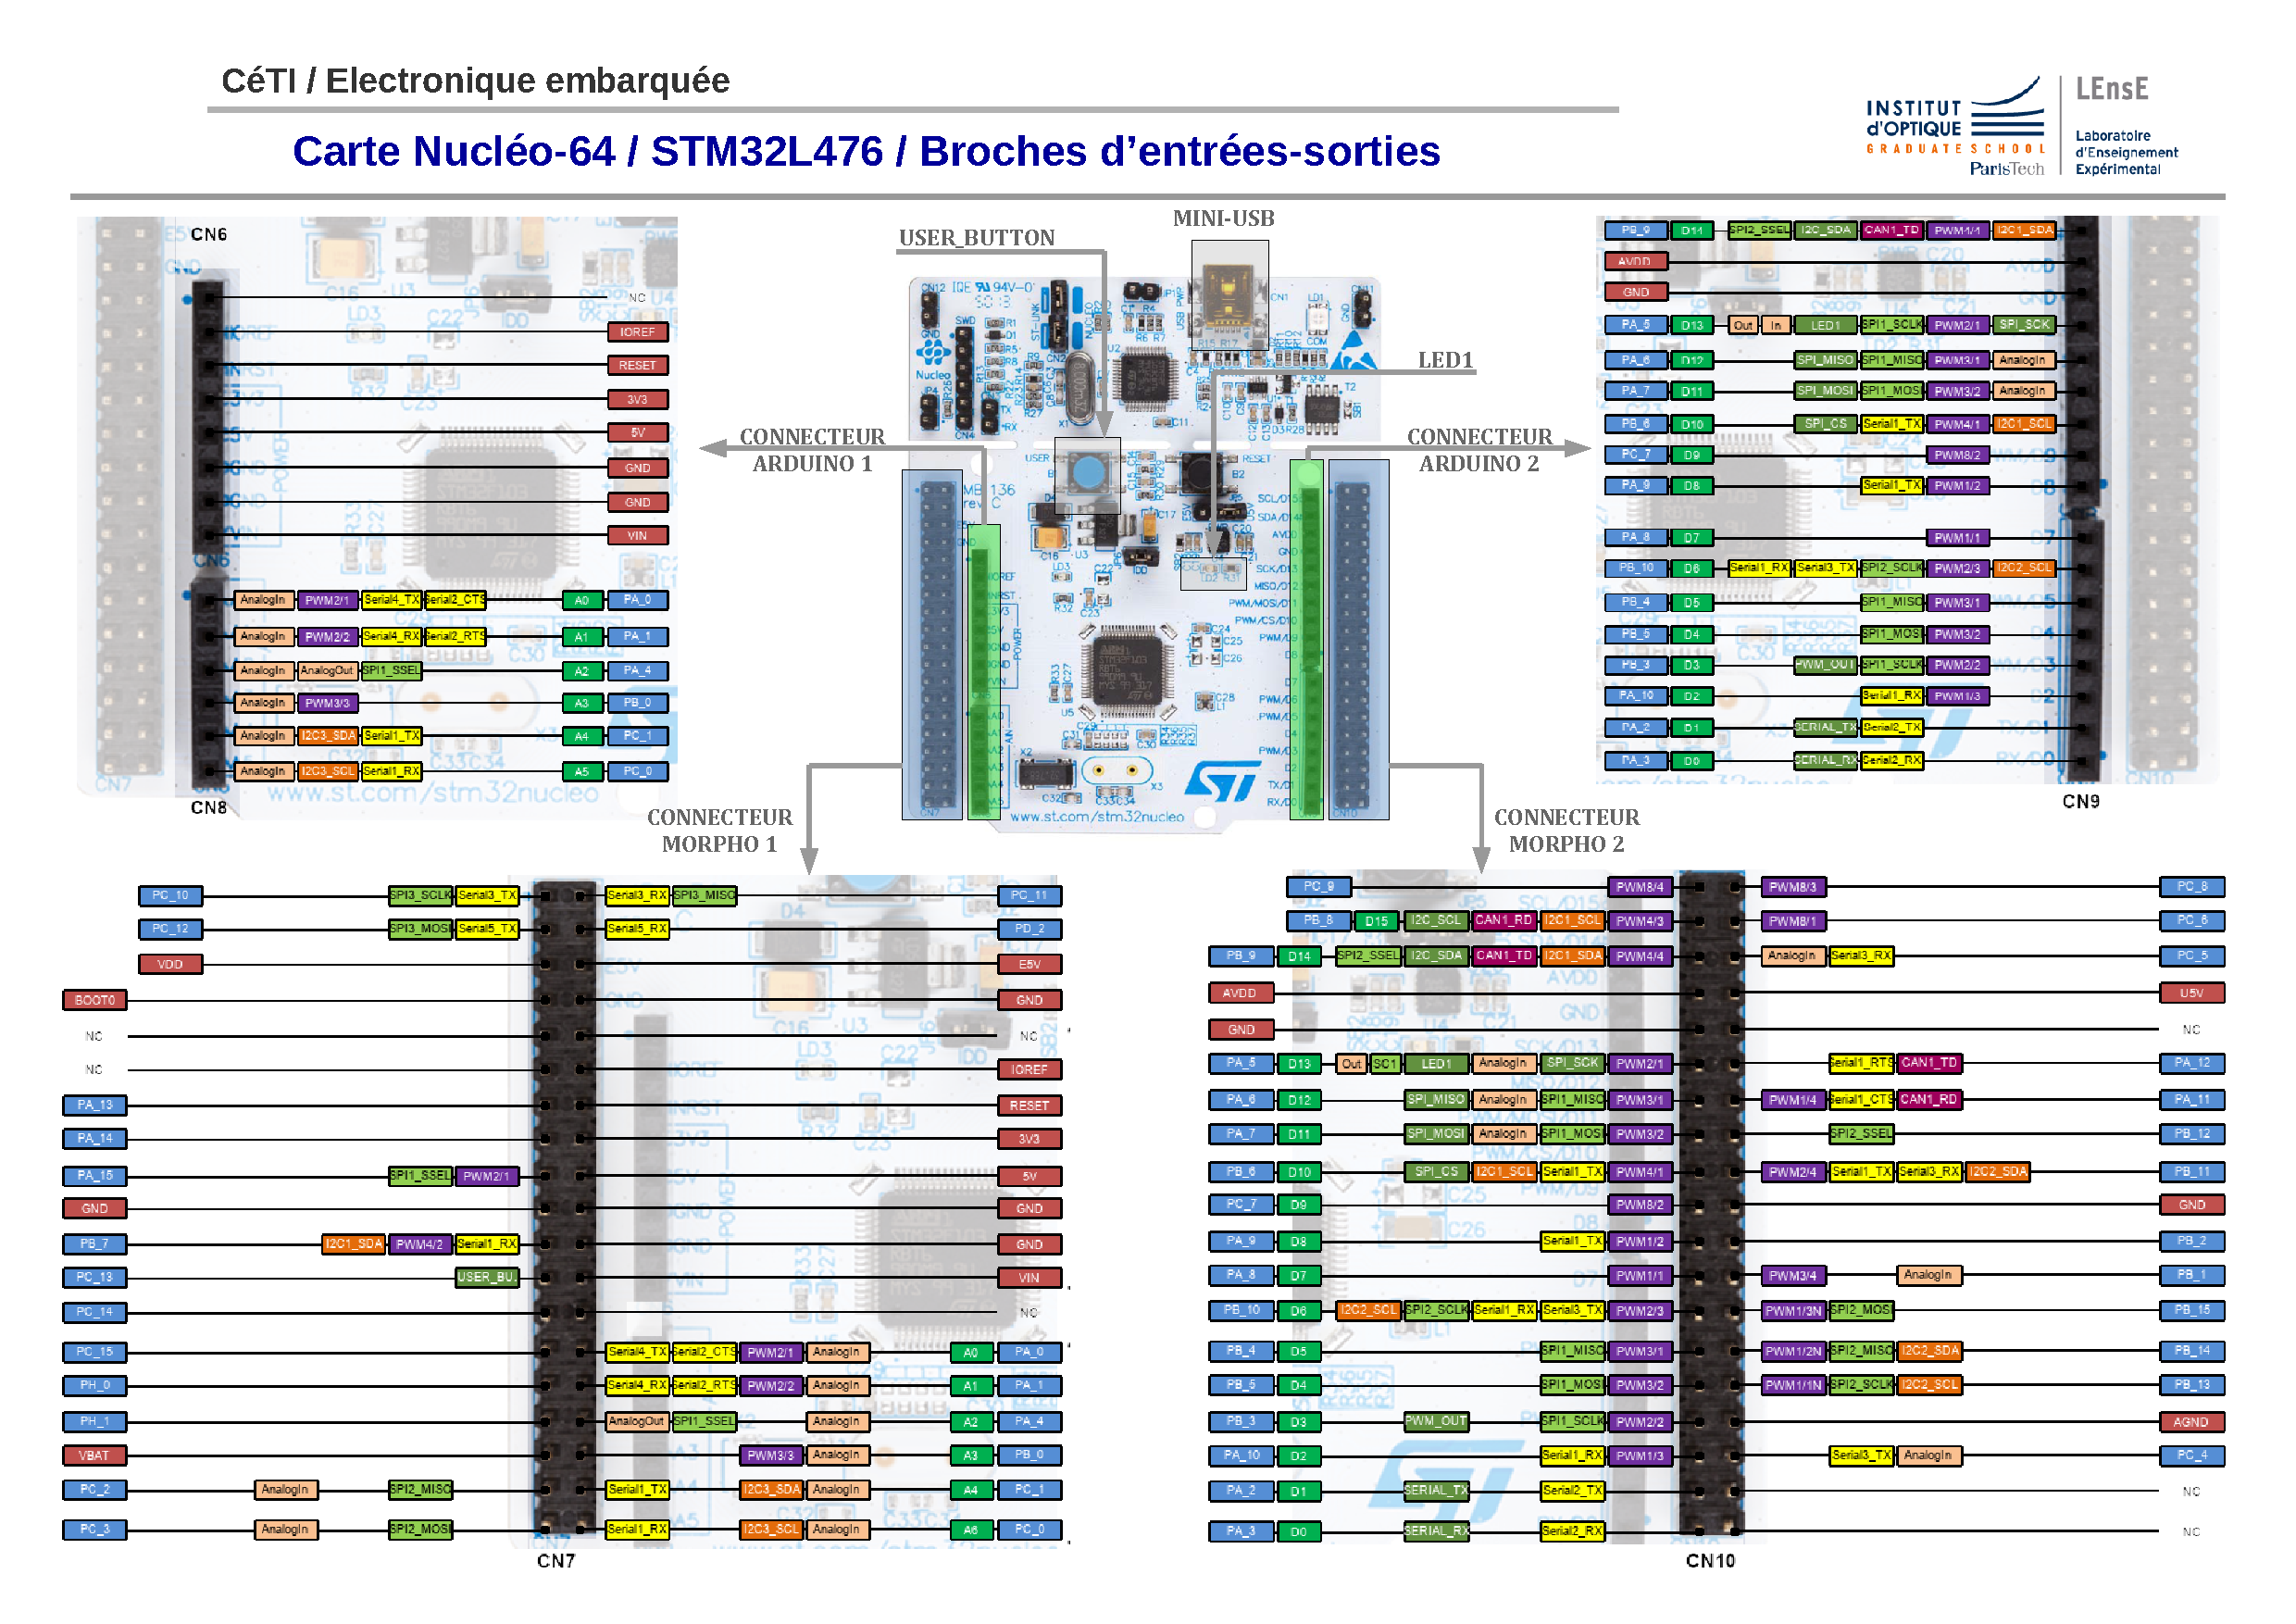
\includepdf[pages=1, landscape=true, pagecommand={\section{\texorpdfstring{\hspace{-1em}}{PCB Robot}}}\label{doc:nucleo_pins_476RG}]{NucleoL476RG_pinout.pdf}

\end{document}


